\chapter{Application Scenario}

This chapter will discuss the information flow of the current system. We will present our understating of the current banking system. we will also give different types of data that exist in the current system and the different operations that are necessary to support the system.
\section{Information Flow}
\begin{figure}[h]
	\centering
	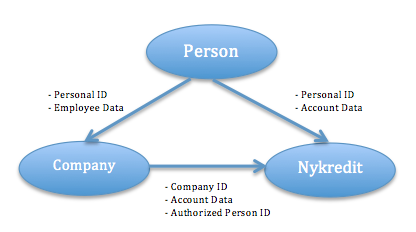
\includegraphics[width=\textwidth]{figures/Flow}
	\caption{Example of information maintained for each relationship}
	\label{fig:Flow}
\end{figure}
A person has different information associated with him. 
\\
\\To Nykredit it can be:
\begin{itemize}
	\item Personal
	 \\This Personal ID can be one of the following identifiers:
	\begin{itemize}
		\item	External ID (e.g. NEMid)
		\item Internal ID (e.g. login credentials of the bank)
	\end{itemize}
\item Account Data
\end{itemize}
To Company it can be:
\begin{itemize}
	\item Personal ID
	\item Employee Data
\end{itemize}
A company has following information that it might share with Nykredit:
\begin{itemize}
	\item Company ID	
	\item Account Data
	\item Authorized Person ID
\end{itemize}
This Authorized Person ID is the identifier that is used by the authorized person on behalf of the company. This can be stored in some database where it is matched to Personal ID of the person.
\\
\\The Authorized Person ID can either be same identifier as the Personal ID, the Company ID or a different identifier that can be authenticated. 
\\
\\In case the Personal ID is used as the Authorized Person ID, it gives Nykredit some additional capabilities:
\begin{itemize}
\item Nykredit can use this information to recruit new customers. If the authorized person is not a customer before, Nykredit can use this info to contact them.
\item If the person is already a customer, then Nykredit can use this information to provide additional services to him on his personal account, so as to influence the authorized person for his decisions regarding the company account (similar to the way airlines reward frequent flyers).
\item As Nykredit already knows about company accounts, the performance of the company might influence their decision regarding the private account of the employee (e.g. it may be difficult for a person to take out a mortgage if Nykredit knows that the company they work for is in financial difficulties).
\item In the case where the customer is accessing Nykredit services on behalf of a smaller financial institution, the capability of matching the authorized ID to Personal ID gives a chance to Nykredit to recruit this customer away from the smaller financial institutions.
\end{itemize}
While good corporate governance at Nykredit will prevent these issues, it is desired to completely and demonstratively remove the link between Personal ID and Authorized Person ID. This, however, creates difficulties with respect to regulatory requirements for accountability at Nykredit and KYC, AML, “Hvidvaskningsloven, etc., so there must be some way to map the identifier used in a financial transaction to a real person, i.e. map a given Authorized Person ID to a Personal ID.

\section{Separation of Identities}
A way to remove the link between Personal ID and Authorized Person ID is to use separate IDs and to maintain a database which links the Authorized Person ID back to the Personal ID. This database can be protected in different ways, so that the information can be used only in case legal authorities need to link the two IDs.
\\
\\This database can be maintained at 3 places :
\begin{itemize}
	\item Company 
	\item Nykredit
	\item Trusted 3rd party
\end{itemize}
\subsubsection{Database on Company Side}
\textbf{Advantages}
\begin{itemize}
	\item Nykredit doesn’t have to invest extra in IT infrastructure
	\\
	\\It is expensive to maintain the entire IT infrastructure by Nykredit, so it is easier and cheaper for Nykredit to let the company maintain the database.
	\item Nykredit can easily prove that it cannot link different Identities
	\\
	\\Nykredit does not have access to the database, so it can easily be proved that Nykredit cannot link the different identities.
	\item Company maintain their own private data
	\\
	\\Companies can be sure that Nykredit does not have access to the personal data of their employees
\end{itemize}
\textbf{Disadvantages}
\begin{itemize}
	
	\item There is no way to retrieve data if the company stops existing
	\\
	\\In this case the entire mapping database may be lost.
	\item Authorities have to go to the Company to get the data
	\\
	\\Nykredit does not have access to the database, so the authorities have to go to Nykredit first to obtain the Authorized Person ID and then to the individual companies next to get the Personal ID.
	\item Company might tamper with the database
	\\
	\\In the case of a rogue employee at the company, which is exactly the case that the legislation is intended to identify, this employee will have easy access to this database and hence the ability to tamper with the database and remove the authorities ability to identify him.
	\item It might prove too difficult for new customers to fulfill all the technical requirements 
	\\
	\\Larger companies can have their own IT infrastructure, but for smaller companies it might prove to be a difficult task to become a new Nykredit customer if they have to invest extra in IT infrastructure just for this purpose.
\end{itemize}

\subsubsection{Database on Nykredit Side}
\textbf{Advantages}
\begin{itemize}
	\item In case the company stops existing, the data can still be retrieved
	\\The database is always with Nykredit, so if some company stops existing, it can still be accessed.
	\item Authorities have a single place to obtain all the data
	\\Authorities do not have to go to individual companies to get the relevant data as everything is at one place.
	\item Company cannot tamper with database
	\\As companies have no direct access to the database, they cannot tamper with it.
\end{itemize}
\textbf{Disadvantages}
\begin{itemize}
	\item Nykredit has to invest extra in IT infrastructure
	\\
	\\Nykredit has to invest extra to keep this system in place.
	\item Company does not have control over their own private data
	\\
	\\The database is on Nykredit side, so companies have to store the data there and hence they do not have control over their own private data.
	\item It is difficult for Nykredit to prove that they cannot link different identities when they are managing the database
	\\
	\\Nykredit will be managing everything in-house, so it is difficult to prove that they cannot access the database and link the identities.
	\item It may be difficult for customers to adhere to the Nykredit technological standards
	\\
	\\Nykredit may not be able to support all available technologies for their customers, so some customers, who are using a different setup than Nykredit, may find it difficult to comply with the Nykredit standard.
\end{itemize}
\subsubsection{Database on 3rd Party Side}
\textbf{Advantages}
\begin{itemize}
	\item Neither companies nor Nykredit have to invest extra in IT infrastructure
	\\
	\\The database is managed by the trusted 3rd party, who will invest in the infrastructure, so neither Nykredit nor the companies will have to invest extra in IT infrastructure
	\item It is easier for new and old customers to be a customer at Nykredit
	\\
	\\The trusted 3rd party can support a wide range of technologies, so it is easier for customers to use their existing technology when becoming a new customer at Nykredit
	\item Nykredit can easily prove that it cannot link different Identities
	\\
	\\Nykredit is not hosting the database, so it is easier for them to prove that they cannot link the identities.
	\item Data can still be retrieved in case the company stops existing 
	\\
	\\The database is always with the trusted 3rd party, so it does not matter if some company stops existing, the data can still be accessed. Special arrangements have to be made in case the trusted 3rd party ceases to exist, but this will be rare and in that case, Nykredit may decide to take over that part of the trusted 3rd party.
	\item Company cannot tamper with database
	\\
	\\The companies do not have access to the database, so they cannot tamper with the data.
	\item Authorities only have to go to the trusted 3rd party to get the data in case its needed.
\end{itemize}
\textbf{Disadvantages}
\begin{itemize}
	\item The 3rd party must be trusted by both Nykredit and its customers
	\\
	\\The database is neither with the company nor Nykredit, so the external service provider should be trusted by both parties to hold their sensitive data.
	\item In case the trusted 3rd party goes out of business it might be difficult to retrieve the data.
	\item Companies do not have control over their own data
	\\
	\\The database is maintained by an external service provider, so the companies have to store the data there and hence they do not have control over their own private data.
\end{itemize}
\section{Current Banking System}
The current banking system can be seen as following.
\begin{figure}[h]
	\centering
	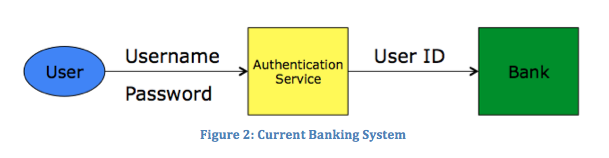
\includegraphics[width=\textwidth]{figures/Current}
	\caption{Current Banking System}
	\label{fig:Current}
\end{figure}
There are 2 parts of the system:
\begin{itemize}
	\item Authentication Service 
	\item Bank
\end{itemize}
The end user interact with the service as follows:
\begin{itemize}
\item User goes to the authentication service and enters his credentials
\item Authentication service authenticate the user and gives the bank User ID of the user
\item All other details of the user are stored at bank side in relation with his user ID
\item Bank provide services to the user 
\end{itemize}
The authentication service can either be controlled by bank or a 3rd party (e.g. NemID)
\\In this system Bank is the most powerful entity. It has all the mappings
\begin{itemize}
	\item User ID $\rightarrow$ Account ID
	\item User ID $\rightarrow$ Policy
	\item User ID $\rightarrow$ User Personal Data
	\item User ID $\rightarrow$ Transactions
\end{itemize}
This makes the bank most powerful identity in the system. Its very easy for bank to get any private data of customers using the data stored on bank side.

In nutshell current banking system gives bank a lot of power over user data. Also we have seen that traditional methods are not sufficient to provide proper anonymity to the users or they don't fit all the requirements properly.